\documentclass[supercite]{upcthesis}
\usepackage{lipsum}
\usepackage{makecell}
\usepackage{amsmath}
\usepackage{mathtools}
\usepackage{amsfonts,amssymb}
\usepackage{subfigure}
\usepackage{enumerate}
\usepackage{graphicx}
\usepackage{epstopdf}
\usepackage{etoolbox}
\usepackage{titlesec}
\usepackage{tocloft}

\usepackage{ntheorem}






\theorembodyfont{\songti}
{
\newtheorem{mdef}{\hskip 2em 定义}[section]  %按一级标题section编号
\newtheorem{mthe}{\hskip 2em 定理}[section]
\newtheorem*{mpro}{\hskip 2em 证明} %不编号
\newtheorem{mlma}{\hskip 2em 引理}[section]
\newtheorem{mcor}{\hskip 2em 推论}[section]
\newtheorem{mprop}{\hskip 2em 命题 }[section]
\newtheorem{mexa}{\hskip 2em 例 }[section]
}


%%%%%%%%%调整subsection与subsubsection格式
\titlespacing*{\subsubsection}{0pt}{0.5ex plus .2ex minus .2ex}{%
	0.5ex plus .2ex
}
\titlespacing*{\subsection}{0pt}{0.5ex plus .2ex minus .2ex}{%
	0.5ex plus .2ex
}
%%%%%%%%%貌似是调整参考文献格式?
\let\oldthebibliography \thebibliography
\let\endoldthebibliography \endthebibliography
%\renewenvironment{thebibliography}[1]{%
%	\begin{oldthebibliography}{#1}%
%		\setlength{\parskip}{0ex}%
%		\setlength{\itemsep}{0ex}%
%		\setlength{\itemindent}{4ex}
%		\setlength{\leftmargin}{-3pt}%
%	}% 
%	{
%	\end{oldthebibliography}%
%}
%%%%%%%%%调整数学公式格式,貌似是设置公式编号格式?
\renewcommand{\theequation}{\thesection -\arabic{equation}}
\makeatletter
%%%%%%%%%貌似是调整参考文献文本格式(如缩进等),非参考文献自身格式
\renewenvironment{thebibliography}[1]
{\section*{\refname}%
	\@mkboth{\MakeUppercase\refname}{\MakeUppercase\refname}%
	\list{\@biblabel{\@arabic\c@enumiv}}%
	{\settowidth\labelwidth{\@biblabel{#1}}%
		\setlength{\itemindent}{\dimexpr\labelwidth+\labelsep}
		\leftmargin\z@
		\@openbib@code
		\usecounter{enumiv}%
		\let\p@enumiv\@empty
		\renewcommand\theenumiv{\@arabic\c@enumiv}}%
	\sloppy
	\clubpenalty4000
	\@clubpenalty \clubpenalty
	\widowpenalty4000%
	\sfcode`\.\@m}
{\def\@noitemerr
	{\@latex@warning{Empty `thebibliography' environment}}%
	\endlist}
%%%%%貌似是数学公式从每个章节(section)重新开始编号
\@addtoreset{equation}{section}
\makeatother

\title{线性表的设计和实现}

\author{张三}
\date{2018年6月1日}
\supervisor{罗\hspace{0.53cm}翔}
\stuid{1401013101}
\classnum{电气工程及其自动化14-5班}
%\subtitle{这是副标题}


%%%%%%%%%%%%%为了让长到换行的标题能够在第一个字的位置对齐,请在断行的位置加上   \\\hspace{4.1em} 


%%%%%%%中英题目
\cntitle{\begin{center}线性表的设计和实现\end{center}}
\entitle{\begin{center}The design and implementation of the linear form\end{center}}
%\ensubtitle{This is EnSubTitle}
\begin{document}
\maketitle
%	\lipsum[1]
\begin{cnabstract}{数据结构;面向对象;可视化;算法;关键字1;关键字2;关键字3;需要换行的关键字}
结构算法设计和演示(C++)树和查找是在面向对象思想和技术的指导下,采用面向对象的编程语言(C++)和面向对象的编程工具(Borland C++ Builder 6.0)开发出来的小型应用程序。它的功能主要是将数据结构中链表、栈、队列、树、查找、图和排序部分的典型算法和数据结构用面向对象的方法封装成类,并通过类的对外接口和对象之间的消息传递来实现这些算法,同时利用C++ Builder 6.0中丰富的控件资源和系统资源对算法实现过程的流程和特性加以动态的演示,从而起到在数据结构教学中帮助理解、辅助教学和自我学习的作用。
\end{cnabstract}


\begin{enabstract}{Write Criterion;Typeset Format;Graduation Project (Thesis);Keyword One;Keyword Two;Keyword Newline}
\lipsum[10]
\end{enabstract}

\tableofcontents

% 加入示例的文章主要部分


\section{引言}
计算机与网络技术的高速发展,特别是面向对象技术的出现,使得C++的软件开发得到了迅速普及。

本课题主要………………




\section{线性表的基本理论知识}
\subsection{线性表的定义}
线性表是最简单、最常用\cite{Rouse1974Monitoring}的一种数据结构。线性表\cite{贾永红2010数字图像处理}是n(n>=0)个数据元素的有限序列。

……。
\subsection{线性顺序表}
线性表的顺序存储结构的特点是为表中相邻的元素$a_i$和$a_{i+1}$ 赋以相邻的存储位置。
\subsubsection{三级标题名}
\subsubsection{三级标题名}
\begin{itemize}
        \item [(1)] 三级以下标题
\end{itemize}




\subsection{线性链表}

线性表的链式存储结构的特点是用一组任意的存储单元存储线性表的数据元素(这组元素可以是连续的,也可以是不连续的)。


\begin{definition}
线性表的定义为
\end{definition}


\begin{theorem}
设sxibaxabxugbuaxbsusabx
\begin{proof}
由线性表的特殊定义可得。
\end{proof}
\end{theorem}
设sxibaxabxugbuaxbsusabx
\begin{lemma}
设sxibaxabxugbuaxbsusabx
\begin{proof}
由线性表的特殊定义可得。
\end{proof}
\end{lemma}



\section{设计的主体内容}
在着手进行上机设计之前首先做好大量准备:应熟悉课题,进行调查研究,收集国内、外资料、分析研究;交互界面的设计和实现。

……。
\subsection{系统结构的设计}
……。
\subsection{交互界面的设计和实现}
交互界面的设计应遵循………。
\begin{equation}
        b\approx\frac{L_0}{\rho\tan(\theta_0)+z_0}
\end{equation}
式中,$z_0$为\textit{Goos-Hanchen}位移;$\theta_0$为光波的入射角。

由公式(3-1)可以看出………。
\subsection{线性表的OOP序设计}
计算机内部可以采用两种不同方法来表示一个线性表,它们分别是顺序表示法和链表表示法。

……。

过阻尼响应如图\ref{guozuni}所示。
\begin{figure}[htbp]
\centering

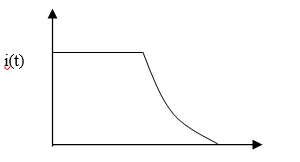
\includegraphics{./figure/guozuni.png}
\caption{过阻尼响应}
\label{guozuni}
\end{figure}
\subsubsection{线性表的顺序存储的实现}
……

以上是顺序表的实现过程,第1-16行包含了list类的说明,接下来是成员函数的定义。

……。
\subsubsection{线性表的链表存储的实现}
……

链表的实现包括两个类定义,第一个是link类,第二个是list类。由于一个链表由若干个单独的链结点对象组成,因此一个链结点应当作为单独的link类实现。

……

……

\section{实验及结果分析}
例如由于起初未能真正掌握各种控件的功能,我设想是要一个下拉菜单,但是学识肤浅的我试了很多种就是达不到我要的效果,……。

……

关于……的影响如表\ref{data_table}所示。

……

\begin{table}[htbp]
        \small
        \newcommand{\tabincell}[2]{\begin{tabular}{@{}#1@{}}#2\end{tabular}}
        \centering
        \caption{激光入射功率密度对导轨滚道表面硬化层深和显微硬度的影响}
        \begin{tabular}{ccccc}
                \toprule
                试验编号 & 功率密度 & 辐照时间 & 显微硬度       & 硬化层深\\ \midrule
                t-1	&6.37×103	&0.067	&570,456	&0.354\\
                t-2	&6.37×103	&0.067	&570,456	&0.354\\
                t-3	&6.37×103	&0.067	&570,456	&0.354\\
                t-4	&6.37×103	&0.067	&570,456	&0.354\\
                t-5	&6.37×103	&0.067	&570,456	&0.354\\ \bottomrule
        \end{tabular}
        \label{data_table}
\end{table}


鉴于表格复杂性,此处提供了可换行示例表见表\ref{kehuanhang}
\begin{table}[htbp]
        \small
        \newcommand{\tabincell}[2]{\begin{tabular}{@{}#1@{}}#2\end{tabular}}
        \centering
        \caption{可换行示例表}
        \begin{tabular}{ccc}
                \toprule
                1	& 2& 3\\ \midrule
                1&\tabincell{c}{3}&6\\
                1&\tabincell{c}{3}&6\\
                \tabincell{c}{2}&\tabincell{c}{4444444444\\5555555555}&\tabincell{c}{6}
                \\ \bottomrule
        \end{tabular}
        \label{kehuanhang}
        \vspace{0.5em}
\end{table}

此处也提供了多列合并示例表如表\ref{duoliehebing}
\begin{table}[htbp]
        \small
        \centering
        \caption{多列合并示例表}
        \begin{tabular}{ccccccccc}
                \toprule
                & \multicolumn{2}{c}{ZZ}& \multicolumn{6}{c}{XX}\\
                \cmidrule(lr){2-3} \cmidrule(lr){4-9}
                &   &   & \multicolumn{2}{c}{CC}&\multicolumn{4}{c}{VV}\\
                \cmidrule(lr){4-5} \cmidrule(lr){6-9}
                &   &   &   &   & \multicolumn{3}{c}{BB}&NN\\
                \cmidrule(lr){6-8} \cmidrule(lr){9-9}
                & A &S	&D &F &G &H &J &K \\ \midrule
                Q&$\surd$&$\surd$&   &   &   &    & &\\
                T&	&		& $\surd$ & $\surd$   &   &  &$\surd$     &\\
                Y&	&		& $\surd$ & $\surd$   &   &  &    &$\surd$ \\ \bottomrule
        \end{tabular}
        \label{duoliehebing}
\end{table}

\section{结论}
        本课题采用C++语言、面向对象的设计方法实现数据结构的重要算法。

        …….

        而且还存在着许多不足之处。如:

% %!TEX option = -shell-escape
\documentclass[supercite,fontset=windows]{upcthesis}



% \def\enEnvironment{} %取消此行注释获得英文环境支持,包括定理环境,交叉引用等
\def \twoSidePrint{} %取消此行注释以获得简单的双面打印效果,在特定位置添加空白页。
\def \eletronicDocument{} %取消此行注释以获得彩色高亮的超链接和交叉引用,便于编写时查看。打印时取消


%导言区设置
%%% 产生一段随机文本的宏包
\usepackage{lipsum}
\usepackage{zhlipsum}


\usepackage{makecell}
%%% 数学环境?
\usepackage{amsmath}
% \usepackage{mathtools}
\usepackage{amsfonts,amssymb}
\usepackage{unicode-math}

%%% 子图
\usepackage{subfigure}

%%% 列表环境
\usepackage{enumitem}
%%% 图片环境
\usepackage{graphicx}

%%%暂时没发现有什么用,注释掉
% \usepackage{epstopdf}
\usepackage{etoolbox}
\usepackage{titlesec}

% 算法/伪代码环境
\usepackage{algorithm}  
\usepackage{algorithmic} 
 % 代码环境
\usepackage{listings}

% \usepackage{tocloft}


%%% 令长表格自动换页的宏包
\usepackage{longtable}


\usepackage{subfiles}
%%%审阅功能
% \usepackage{changes}
%%%交叉引用宏包,要放在最后引入
\usepackage{hyperref}







%%%%%---------------------------------------------------------------------
%%% 定义定理环境的宏包
\usepackage{amsthm}
% 中英定理类环境的声明

% 定义定理样式
\newtheoremstyle{thesty}
{3pt} %环境前间距
{3pt} %环境后间距
{\songti} %定理内字体
{2em} %头部缩进
{\bfseries\songti} %定理头部字体
{} %头部后添加符号
{0.5em} %头部后间距
{} %theorem head spec

% 应用定理样式
\theoremstyle{thesty}

\ifx\enEnvironment\undefined
% 中文定理环境
{
	\newtheorem{definition}{定义}[section]
	\newtheorem{theorem}{定理}[section]
	\newtheorem{lemma}{引理}[section]
	\newtheorem{proposition}{命题}[section]
	\newtheorem{corollary}{推论}[section]
	\newtheorem{example}{例}[section]
	\newtheorem{remark}{注}[section]
}
\newenvironment{proofenv}[1]{\par\indent\songti\textbf{#1}\hspace{0.3em}}{}
\renewenvironment{proof}{\begin{proofenv}{证明:}}{\end{proofenv}\newline \rightline{\qedsymbol}\par}
\newenvironment{solution}{\begin{proofenv}{解:}}{\end{proofenv}}

\else

%% 英文定理环境
{
	\newtheorem{theorem}{Theorem}[section]
	\newtheorem{lemma}{Lemma}[section]
	\newtheorem{proposition}{Proposition}[section]
	\newtheorem{corollary}{Corollary}[section]
	\newtheorem{definition}{Definition}[section]
	\newtheorem{example}{Example}[section]
	\newtheorem{remark}{Remark}[section]
}

\newenvironment{proofenv}[1]{\par\indent\songti\textbf{#1}\hspace{0.3em}}{}
\renewenvironment{proof}{\begin{proofenv}{Proof:}}{\end{proofenv}\newline \rightline{\qedsymbol}\par}
\newenvironment{solution}{\begin{proofenv}{Solution:}}{\end{proofenv}}

\fi


%%%%%---------------------------------------------------------------------

% 交叉引用样式
\ifx \enEnvironment \undefined
%%%--------------------------中文环境引用名
\def\sectionautorefname~#1\null{%
	第~#1~节\null
}
\def\subsectionautorefname~#1\null{%
	第~#1~小节\null
}
\def\subsubsectionautorefname~#1\null{%
	第~#1~小节\null
}

\def\paragraphautorefname~#1\null{%
	段落~#1~\null
}
\def\subparagraphautorefname~#1\null{%
	段落~#1~\null
}

% 重新设置图表 auto ref
\def\figureautorefname~#1\null{%
	图~#1~\null
}
\def\tableautorefname~#1\null{%
	表~#1~\null
}

% 重新设置公式autoref
\def\equationautorefname~#1\null{%
	式~(#1)~\null
}


\def \definitionautorefname~#1\null{
	定义~#1~\null
}
\def \theoremautorefname~#1\null{
	定理~#1~\null
}
\def \corollaryautorefname~#1\null{
	推论~#1~\null
}
\def \lemmaautorefname~#1\null{
	引理~#1~\null
}
\def \propositionautorefname~#1\null{
	命题~#1~\null
}
\def \exampleautorefname~#1\null{
	例~#1~\null
}
\def \remarkautorefname~#1\null{
	注~#1~\null
}
\def \algorithmautorefname~#1\null{
	算法~#1~\null
}

\else

%%%--------------------------英文环境引用名

\def\sectionautorefname~#1\null{%
	Section~#1~\null
}
\def\subsectionautorefname~#1\null{%
	Subsection~#1~\null
}
\def\subsubsectionautorefname~#1\null{%
	Subsubsection~#1~\null
}

\def\paragraphautorefname~#1\null{%
	Paragraph~#1~\null
}
\def\subparagraphautorefname~#1\null{%
	Paragraph~#1~\null
}


% 重新设置图表 auto ref
\def\figureautorefname~#1\null{%
	Figure~#1~\null
}
\def\tableautorefname~#1\null{%
	Tbale~#1~\null
}

% 重新设置公式autoref
\def\equationautorefname~#1\null{%
	Equation~(#1)~\null
}



\def \definitionautorefname~#1\null{
	Definition~#1~\null
}
\def \theoremautorefname~#1\null{
	Theorem~#1~\null
}
\def \corollaryautorefname~#1\null{
	Corollary~#1~\null
}
\def \lemmaautorefname~#1\null{
	Lemma~#1~\null
}
\def \propositionautorefname~#1\null{
	Proposition~#1~\null
}
\def \exampleautorefname~#1\null{
	Example~#1~\null
}
\def \remarkautorefname~#1\null{
	Remark~#1~\null
}
\def \algorithmautorefname~#1\null{
	Algorithm~#1~\null
}


\captionsetup[figure]{name={Figure}}
\captionsetup[table]{name={Table}}
\fi











%%%%%---------------------------------------------------------------------

% 单双面打印控制

\ifx \twoSidePrint \undefined
    \def \ClearPageStyle{\clearpage}
\else
    \def \ClearPageStyle{
    		\clearpage
	    	\thispagestyle{empty}
	    	\quad
	    	\clearpage
    }
\fi

\newcounter{startpage}
\newcounter{endpage}
\setcounter{startpage}{1}
\setcounter{endpage}{1}

\newenvironment{PrintMode}{
	\clearpage
	\setcounter{startpage}{\value{page}}
}{	
	\clearpage
	\setcounter{endpage}{\value{page}}
	% \thestartpage
	% \theendpage
	\addtocounter{endpage}{\value{startpage}}

	\ifodd \value{endpage}
		\ClearPageStyle
		\ifx \twoSidePrint \undefined
		\else
			\addtocounter{page}{-1} % 如果环境内补了一页空白页,将实际页码减一
		\fi
	\fi
}

\newcommand \PrintModeSubfile[1]{\begin{PrintMode}\subfile{#1}\end{PrintMode}}



%%%%%---------------------------------------------------------------------


\ifx \eletronicDocument \undefined

\else
\hypersetup{
	% backref = page,
	% pagebackref = true,
	colorlinks = true,
	linkcolor = blue,
	citecolor = blue,
	urlcolor = blue,
	pdfborder = 000, %去掉链接红(黑)框
	% bookmarks = true,
	% bookmarksopen = true,
	bookmarksnumbered = true
}
\fi

%%%%%---------------------------------------------------------------------
% 代码设置
\lstset{
    % basicstyle          =   \sffamily,          % 基本代码风格
    % keywordstyle        =   \bfseries,          % 关键字风格
    commentstyle        =   \rmfamily\itshape,  % 注释的风格,斜体
    % stringstyle         =   \ttfamily,  % 字符串风格
    flexiblecolumns,                % 别问为什么,加上这个
    numbers             =   left,   % 行号的位置在左边
    showspaces          =   false,  % 是否显示空格,显示了有点乱,所以不现实了
    numberstyle         =   \zihao{-5}\ttfamily,    % 行号的样式,小五号,tt等宽字体
    showstringspaces    =   false,
    captionpos          =   t,      % 这段代码的名字所呈现的位置,t指的是top上面
    % frame               =   lrtb,   % 显示边框
     breaklines      =   true,   % 自动换行,建议不要写太长的行
    columns         =   fixed,  % 强制等宽字体,更美观
}


% 列表宏包样式
\setlist{noitemsep}

\setmathfont{Cambria Math}


% 表格设定
% 添加复杂的表格宏
\usepackage{booktabs}
% 设置三线表格式
\setlength{\heavyrulewidth}{1.5pt}
\setlength{\lightrulewidth}{0.5pt}
\setlength{\cmidrulewidth}{0.5pt}
\setlength{\aboverulesep}{0pt}
\setlength{\belowrulesep}{0pt}
\setlength{\abovetopsep}{0pt}
\setlength{\belowbottomsep}{0pt}







% 封面各项参数
\makeatother
\title{线性表的设计和实现}
\subtitle{这是副标题}
% \ensubtitle{This is EnSubTitle}
\entitle{The design and implementation of the linear form}
\author{张\hspace{0.53cm}三}
\date{\today}
\supervisor{罗\hspace{0.53cm}翔}
\stuid{1401013101}
\classnum{电气工程及其自动化14-5班}




\begin{document}
%%%%%---------------------------------------------------------------------
% 封面页
\maketitle
\ClearPageStyle

% 中文摘要
\subfile{sections/before/cnabstract}
\ClearPageStyle

% 英文摘要
\subfile{sections/before/enabstract}
\ClearPageStyle


% 目录页
\tableofcontents

\ClearPageStyle   % 如果你的目录总页数是偶数,注释掉这一行。否则双面打印时正文的第一页会是空白页

% 防止添加空白页导致的页码出错
\setcounter{page}{1}

%%%%%---------------------------------------------------------------------
% 正文从这里开始


%%% word模板的实现,写自己的论文时注释这里
% \PrintModeSubfile{sections/test/examplesec1.tex}
% \PrintModeSubfile{sections/test/examplesec2.tex}
% \PrintModeSubfile{sections/test/examplesec3.tex}
% \PrintModeSubfile{sections/test/examplesec4.tex}
% \PrintModeSubfile{sections/test/examplesec5.tex}

%%%%%---------------
%%% 测试各种环境,写自己的文时注释这里
% \PrintModeSubfile{sections/test/test.tex}

%%%%%---------------
%%% 使用手册,请编译后认真阅读。写自己的论文时注释这里



\PrintModeSubfile{sections/manual/section1.tex}
% \PrintModeSubfile{sections/manual/section2.tex}
% \PrintModeSubfile{sections/manual/section3.tex}
% \PrintModeSubfile{sections/manual/section4.tex}
% \PrintModeSubfile{sections/manual/section5.tex}
% \PrintModeSubfile{sections/manual/section6.tex}
% \PrintModeSubfile{sections/manual/section7.tex}
\PrintModeSubfile{sections/manual/section8.tex}
%%%%%---------------

%%% 你的章节,使用时按需要取消注释
% \PrintModeSubfile{sections/body/section1.tex}
% \PrintModeSubfile{sections/body/section2.tex}
% \PrintModeSubfile{sections/body/section3.tex}
% \PrintModeSubfile{sections/body/section4.tex}
% \PrintModeSubfile{sections/body/section5.tex}











%%%%%---------------------------------------------------------------------
% 设置页眉为空
\pagestyle{afterbody}

% 感谢页
\PrintModeSubfile{sections/after/thankpage}

% 参考文献页
\PrintModeSubfile{sections/after/reference}

%附录,不需要的同学可以注释此部分
\PrintModeSubfile{sections/after/appendix}

\end{document}


\begin{thankpage}
        大学四年的学习生活即将结束,在此,我要感谢所有曾经教导过我的老师和关心过我的同学,他们在我成长过程中给予了我很大的帮助。本文能够成功的完成,要特别感谢我的导师XXX教授的关怀和教导。

        ……
\end{thankpage}




%\bibliography{./bibs/bibliography.bib}

%%%%%之前的.bib生成引用的样式与word要求不一致。能力有限,暂时无法修改
%%%%%样式文件不同于学校的要求。劳烦同学们手动引用文献

%%%%%手动指定在目录添加参考文献条目
\clearpage
\pagestyle{afterbody}
\phantomsection
\addcontentsline{toc}{section}{参考文献}

% 按照学校word模板中对参考文献的要求,列出以下几点给同学们参考


% 列出的参考文献必须在正文中有引用,并且需按正文中出现的次序进行排序。同一文献出现多次,只用同一标号

% 参考文献里的标点符号均为英文格式输入,每个标点符号与后面的内容之间要空一格。参考文献的各项条目使用逗号分割,最后要有句点。


% 参考文献应不少于10篇(外文文献至少2篇,外语专业应以外文文献为主)。

% 文献引用的格式大致为:

% 作者1, 作者2, 作者3, et. al, 题目, 期刊, 时间, 期数(卷数), 起-始页,网址.

% 其中不那么重要的或没有的部分可不写
% 其中:

% 英文作者,名缩写(老外是名在前,姓在后),如:Robert Jort缩写为:R. Jort,名字两个单词的,G. H. Golub。作者太多不适合全部列出的,写上 et. al,

% 英文题目除专有名词外,仅第一个单词首字母大写
% 题目中表示文献类型的符号:[M] [J] 等一律删掉,不允许出现。
% 期刊名应写全称,不知道的可以上网搜索。英文期刊中实词首字母的写。
% 一些英文常见期刊:

% 日期统一改为如下格式 2003.5.12


\begin{thebibliography}{99}
\bibitem{1} 严蔚敏, 吴伟民, 数据结构, 北京: 清华大学出版社, 1997.4.
\bibitem{2} 沈晴霓, 聂青, 苏京霞, 现代程序设计—C++与数据结构面向对象的方法与实现, 北京: 北京理工大学出版社, 2002.8.
\bibitem{3} T. Connolly, C. Begg, Database systems, 北京: 电子科技工业出版社, 2004.7.
\bibitem{4} R. Bate, S. Shrum, CMM Integration framework, CMU/SEI Spotlight, 1998, 4(3): 25-28.
\bibitem{5} J.P. Kuilboer, N. Ashrafi, Software process and product improvement, Physical Review A, 2000, 42(1): 27-34.
\bibitem{6} 张美金, 吴大伟, 基于ASP技术的远程教育系统体系结构的研究, http://172.50.0.88:86 /~cddbn/Y517807/pdf/index.htm, 2003-05-01.
\bibitem{7} 王伟国, 刘永萍, 王生年等, B/S模式网上考试系统分析与设计, 石河子大学学报(自然科学版), 2003, 6(2): 145-147.
\bibitem{8} …
\bibitem{9} …
\bibitem{10} …
\end{thebibliography}




%%%%%%%%附录,不需要的同学可以删去此部分

\begin{generalappendices}
        \section{名词术语及缩略词}
        \subsection{Some Appendix}
        \lipsum[11]
        \section{Appendix 2}
        \subsection{Some Other Appendix}
\end{generalappendices}
\end{document}